
\section*{Discussion}

Now that we have seen two commercial, integrated security chips (Titan and T2) and two user-attachable, research tokens (\protection and \proximitee), we can can discuss their deployment aspects, security benefits and previous comparable solutions. 

\paragraph{Deployment options}
Integrated security chips like Titan and T2 are, obviously, limited to deployments by major service and platform providers that have the possibility to design and build their own systems. 

\proximitee is an example of a plug-and-play security token that can be attached to the target platform over a standard interface like USB. Deployment of security solutions is a feasible option for a larger set of service providers. For example, cloud computing providers can enhance off-the-shelf servers with \key tokens and communicate their public keys to their clients to support more secure attestation. Another interesting use case is the setup of a permissioned blockchain where every consensus node is hardened with SGX enclaves. The trusted authority that appoints the consensus nodes can issue a \key token to each organization that operates one node.

Also \protection could be deployed as a plug-and-play security module. Such deployment allows service providers like voting authorities and banks to increase the security of their services without restricting the users' choice of client platform. In medical and industrial domains, an externally-attached \protection module can improve the security of safety-critical systems, even when modifications to the computing platform itself are prohibited due to strict regulations. Alternatively, \protection could be deployed as an integrated security chip such that its functionality is implemented as part of the integrated keyboard, mouse, and display controllers. 

%\begin{figure}[t]
%    \centering
%    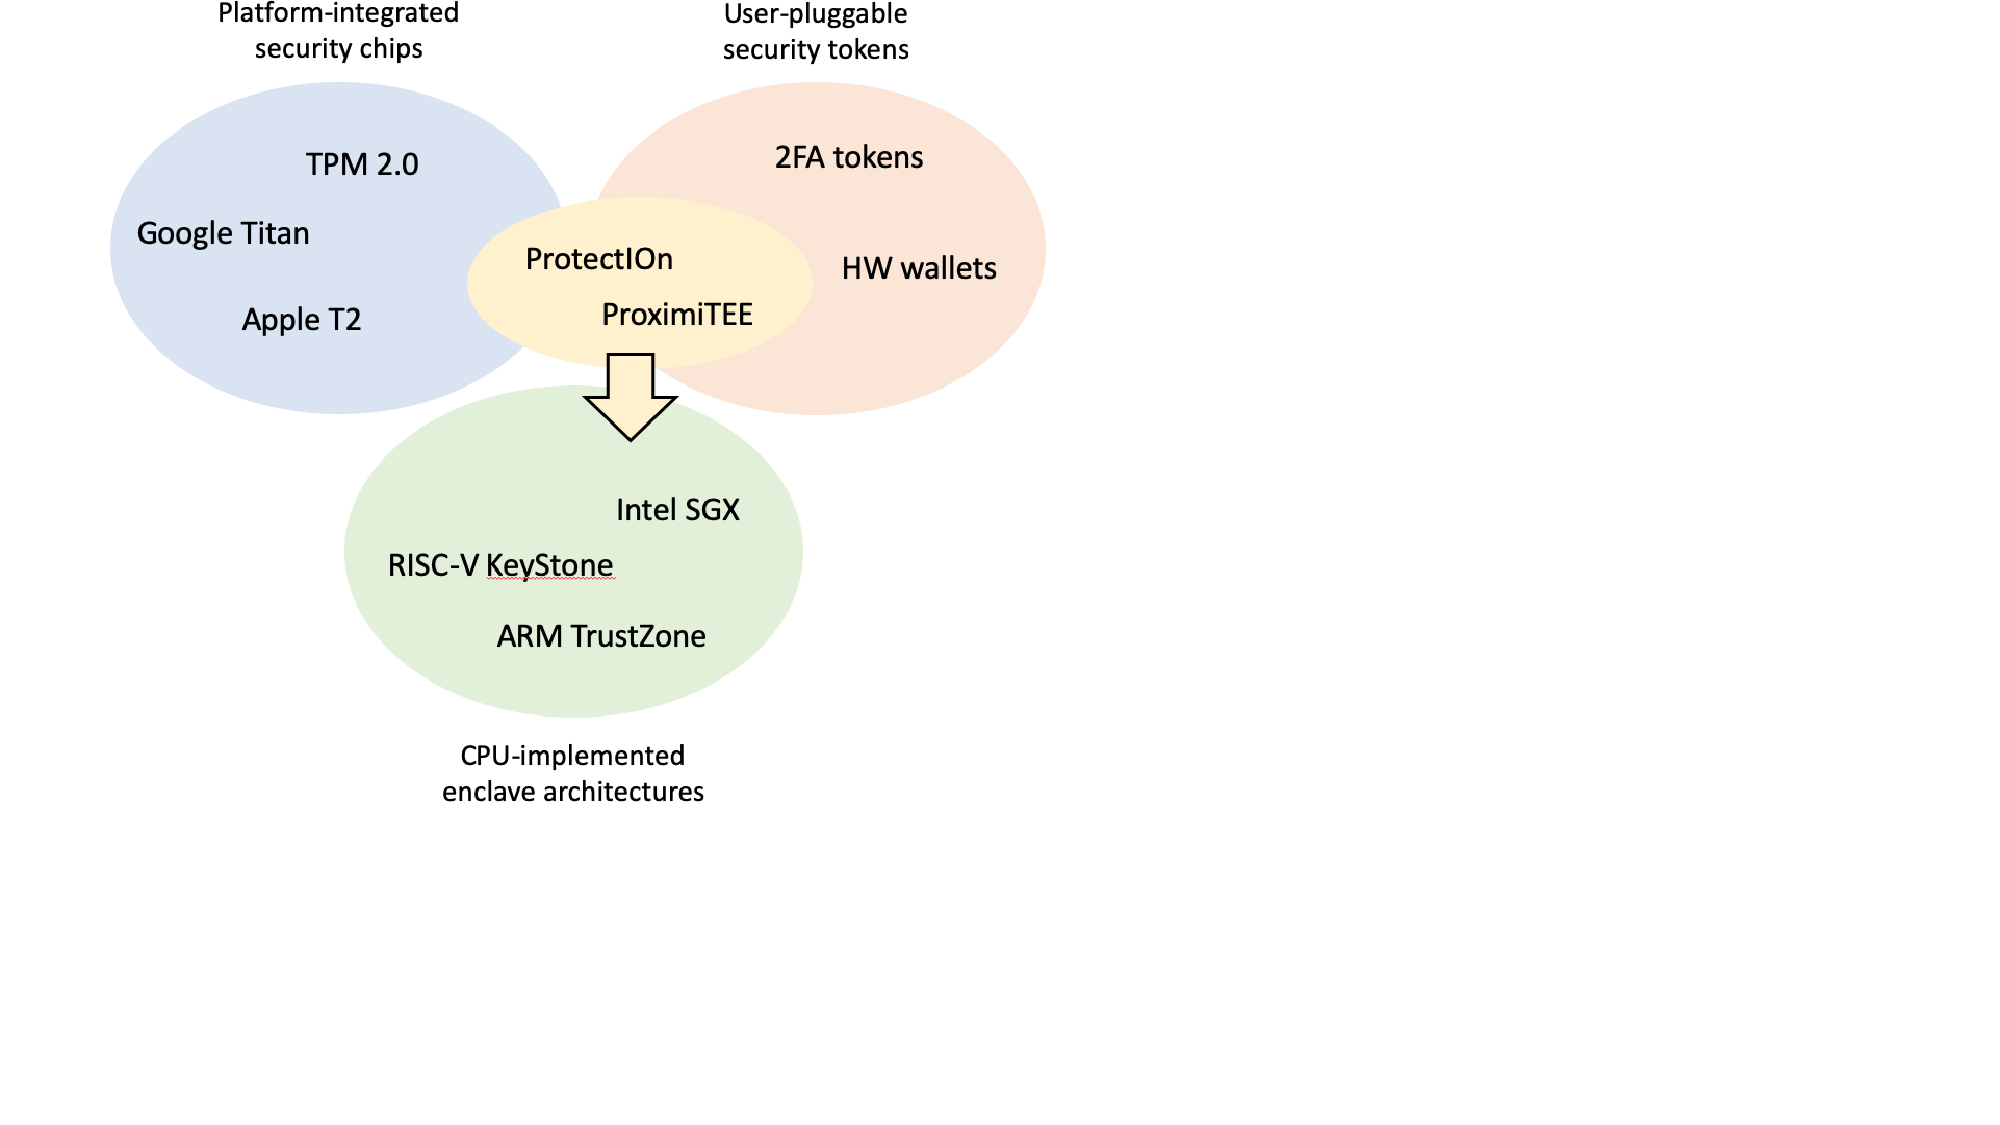
\includegraphics[scale=0.4]{comparison.pdf}
%    \caption{Comparison of \protection and \proximitee with respect to the platform-integrated security chips, user-pluggable security tokens and CPU-implemented enclave architecture.}
%\label{fig:prototype}   
%\end{figure}

\paragraph{Security benefits}
Titan and T2 are chips that enable security functionality like a secure boot that is not provided by enclaves. Thus, the operation of Titan and T2 is largely orthogonal to the operation of enclaves. 

In comparison, \proximitee is a security chip that is designed to work in collaboration with enclaves and improve their security guarantees by enabling secure TEE identification for hardened remote attestation. 

\protection is a solution that can either assist enclaves or operate independently of them. One possible usage for \protection is to enable a trusted path from the user to a local enclave, which can communicate securely with remote servers. In such a deployment, \protection works together with an enclave. 
%
Alternatively, \protection could be used to create a trusted path from the user to a remote server without the use of enclaves. Such deployment is beneficial when the risk of microarchitectural attacks on enclaves is considered too high, for example.


\paragraph{Dedicated chips and early TEEs}

\update{5}{\protection and \proximitee are systems where a dedicated chip complements and improves the security guarantees of enclaves. Some previous TEE designs have leveraged dedicated security chips to implement the TEE itself.}

\update{5}{AMD's Secure Virtual Machine technology is one such example where the TEE is created as follows: the CPU measure code in a specific memory region, enables DMA protections for that region, disables interrupts, records the measurement into a PCR register of a TPM chip, and finally begins executing the measured code. Essentially, this sequence of events provides a clean execution of the measured code without restarting the whole platform, and therefore this technology is often called ``late launch''. The main role of the dedicated chip (TPM in this case) is to securely record the code that was launched so that an external verifier can check its integrity using attestation.}

